
\subsubsection{Microelectronics}\label{ict:micro:bergholz}
\index{Bergholz, Werner}

\paragraph{Research Team}
Werner Bergholz (Professor), Thomas Dinkel (PhD student), Uwe Pagel (Technical
Assistant)\\

%%% give a very short (150 words description of your research area)
%% Hint: this can be copied from the research areas document (../masterplan/research-areas)

After 30 years of rapid advancements in microelectronics barriers are emerging for a
further device shrink and/or improvement of quality/failure rates. Our research focuses on
these ``brick walls''. These barriers are mainly related to defects, which limit yield and
reliability and the exploding cost for lithography. In addition, nanotechnology artefacts,
such as carbon nano tubes and quantum dots are getting closer to integration into
conventional microelectronic products. The specific research topics are the
\begin{myitemize}
\item Development of destruction free methods to detect defects in silicon wafers
\item Defect-related failure mechanisms and reliability test methods for microelectronic
  circuits.
\item New wafer types with functional layers to mitigate the cost explosion for
  lithography
\item Novel process control methodology to improve quality and productivity.  Unless
  solutions for the listed challenges can be identified, the rapid expansion of
  information technology will slow down within the next 5 years.  In addition, the
  following additional research topics are being addressed,
\item Investigation of defect engineering methods and efficiency detractors in Si solar
  cell technology (based on an synergy with microelectronics techniques)
\item Application of Quality Management methodology and standardisation techniques to
  nanotechnology and other non-technical areas.
\end{myitemize}
One of the more subtle limitations to further device shrink is a phenomenon known as
random telegraph signals (RTS noise) in semiconductor devices. Known and not understood
for more than 30 years, it never had particular technological importance. With devices in
the 100nm size range or below, it is gradually transforming from a laboratory curiosity to
a serious challenge in many application areas.

\begin{figure}[ht]
  \begin{center}
      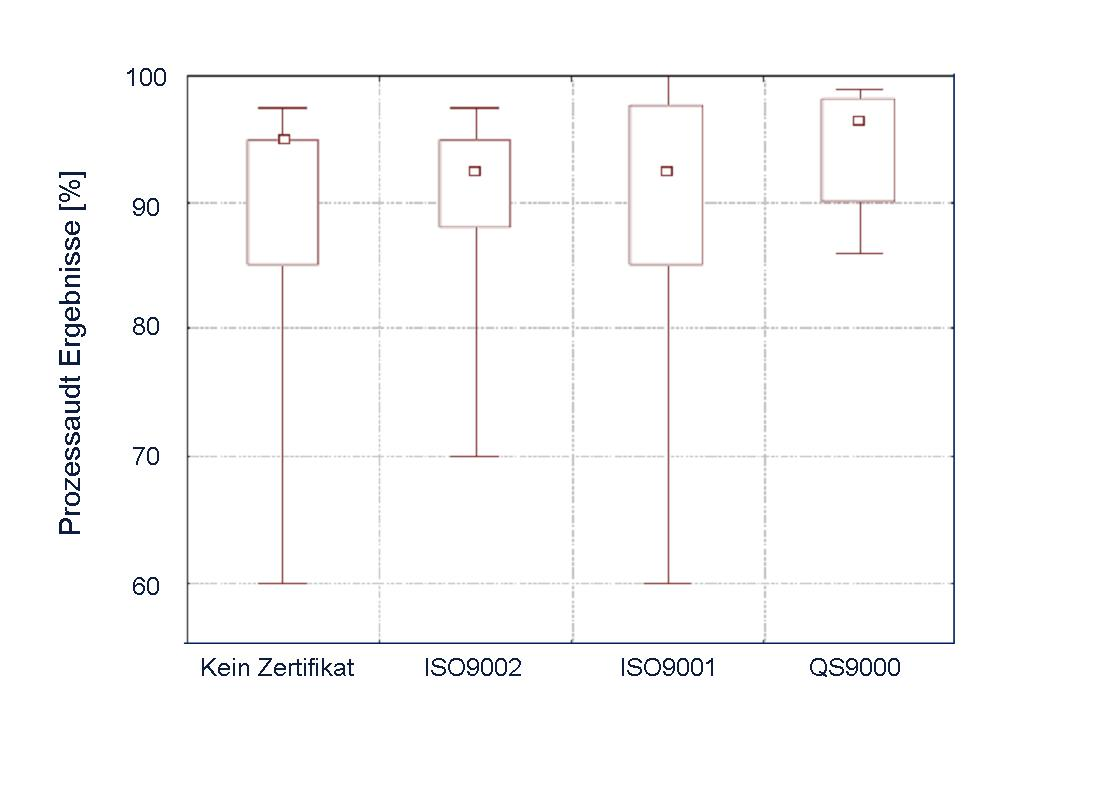
\includegraphics[width=\hsize]{EECS/bergholz-fig1}
    \mycaption{Boxplot comparison of the scores in a process-oriented audit of suppliers
      to the microelectronics industry. Suppliers which conform to the QS9000 (TS16949)
      Quality standard are clearly superior to ISO9000 certified or not certified
      companies}
    \label{fig:switching}
   \end{center}
\end{figure}

\paragraph{Highlights}

{\emph{Quality Management methodology}}: An evaluation of about 100 second party audits of
materials suppliers to the microelectronics industry has shown that a certification
according to the quality management standard TS16949 (formerly QS9000) correlates with
positive results in a process oriented audit methodology (see Fig.~\ref{fig:switching}). On
the other hand, certification according to the standard ISO9001 and ISO9002 (less
stringent than TS16949) does not guarantee a sufficient quality level, if it is compared
to the former group or companies which have no certification at all. There are also
significant differences between silicon wafer manufacturers (which have a decade long
tradition in clean room technology and high quality standards) and producers of other
materials for the Chip industry (chemicals, gases, metals etc.). Furthermore, it can be
concluded that the process oriented audit methodology is a sutiable tool to measure the
quality standard of a
supplier.\\

{\emph{Random Telegraph Signals in Si devices}}: The study of random telegraph signals in
diodes has been extended to the influence of temperture bias stress measurements
(S. Nandhavel \& W. Bergholz). After 175 degrees C (Fig.~\ref{fig:leakage}) leakage can be
observed, which is consistent with the hypothesis that metal boron pairs are the
responsible defects. Deep Level Transient Spectroscopy, radiation experiments and TEM
studies are planned to track down the defect mechanism.

{\emph{Photovoltaics industry}}: A systematic study of the open data for the process
capabilities of all major PV manufacturers has revealed an unexpected large variation in
the efficiencies and other performance indicators. It is planned to identify methods how
the process variation can be reduced by "copy intelligently" of engineering methods
developed in the microelectronics industry.

\begin{figure}[ht]
  \begin{center}
    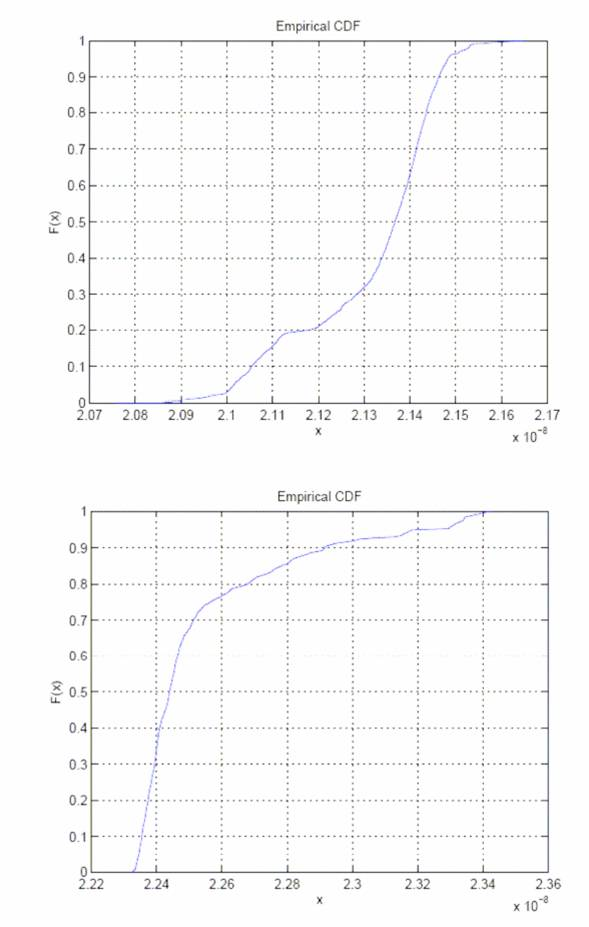
\includegraphics[width=7cm]{EECS/bergholz-fig2}
    \mycaption{After temperature bias stress of a diode there is a reversible recovery of
      the leakage currents for voltages slightly below the barrier voltage, attributed to
      diffusion pairing reactions of metal impurities, comparison of the cumulitive
      distribution function for the leakage curents before and after stress at 175 degrees
      C}
    \label{fig:leakage}
   \end{center}
\end{figure}

{\bf Outlook}: It is planned to supplement the study on audit methodology to a correlation
with a performance evaluation of the same suppliers and to extend the study to the data
gathered by a major car manufacturer in about 10 000 quality audits at suppliers to the
car industry. Objective: further refine the audit methodology and quality management
implementation methods. The Study on RTS will be extended to the investigation of methods
to reduce the effect and thus lower or remove one of the roadblocks to the
microelectronics industry. The long term goal of the PV studies is to develop efficient
defect reduction and efficiency optimization methods so as to support the goal for cost
reduction by a factor or 3 until PV becomes competive for peak power in grid
applications. The standardisation research in cooperation with DIN, DKE and SEMI is
targetted towards early anticipatory standards in emerging nanotechnology to facilitate
the transformation from lab to fab.

%\newpage
\paragraph{Organization}
\begin{enumerate}
\item Workshop: ``Silicon Wafers SEMI� Standards Workshop'', April 05 2006, Munich Trade
  Center
\item SEMI Autumn Conference: ``Conference "Bridging Semiconductor \& Related'', 08th
  Nov2006 Dresden
\end{enumerate}
\paragraph{Collaborations}
\begin{enumerate}
\item {\sl Infineon Technologies, Dresden}\\
  RTS noise phenomena
\item {\sl Infineon Technologies, Munich}\\
  Test Set up for DRAMs
\item {\sl MEMC, St. Peters, Missouri}\\
  Defect Detection in Silicon Wafers
\item {\sl Q-Cells, Thalheim}\\
  Efficiency Engineering for Silicon-based Solar Cells
\item {\sl Quintiq, S'Hertogenboch, Netherlands}\\
  Best practice Quality Management Tools for the Software Industry
\item {\sl International University Bremen}\\
  Dietmar Knipp\\
  Solar cells, low cost electronics
\item {\sl International University Bremen}\\
  Peter Ludes (SHSS), C. Schwender (JCLL)\\
  Visual mass communication
\item {\sl SEMI (Semiconductor Equipment and Materials)
    San Jose, Brussels}\\
  Bettina Weiss, Carlos Lee\\
  Semiconductor Standards Development
\item {\sl DIN, Berlin}\\
  Standardization of Nanomaterials
\item {\sl DKE, Frankfurt, Main}\\
  Standarization of Nanoelectronic Electronic Products
\end{enumerate}

\paragraph{Patents}
\begin{enumerate}
\item Patent on wafer technology, in the filing process
\end{enumerate}

\paragraph{Grants}
 \begin{enumerate}
\item Funded by Deutsches Institut f�r Normung (DIN/DKE) /
Bundesministerium f�r Wirtschaft,  \emph{Standardisierung
Nanoelektronik} (July - December 2006)
\end{enumerate}

\paragraph{Awards, Prizes}
\begin{enumerate}
\item shortlisted for the IEC centinary Award Challenge
\end{enumerate}

\newpage
%\paragraph{Publications}
%\nocite{BerWeiLee:QFD05}
%\nocite{KumWeiPagBer:ecrtnd05}
%\nocite{BaaBerg:ddf05}
\nocite{WittBerg:wbqz06}
\nocite{Berg:msinpb06}
\nocite{BergWeLee06}


%\end{description}
%\end{document}
%%% Local Variables:
%%% mode: latex
%%% TeX-master: "report"
%%% End:
